\title{Operating Systems–1: CS3510 Autumn 2018\\
Programming Assignment 2: \\
Multi-Threaded Computation of Statistics\\
Report}
\author{Sai Harsha Kottapalli}
\date{November 26, 2018}

\documentclass[12pt]{article}
\usepackage{graphicx}

\begin{document}
\maketitle

\section{Aim}
The goal of this assignment is to compute some statistics over a sequence of input numbers
using multiple threads, processes and compare the times taken by each of them.

\section{Explanation of program(Multi-Process)}

\subsection{mmap()}
mmap() creates a new mapping in the virtual address space of the calling process. \\

If addr is NULL, then the kernel chooses the (page-aligned) address at which to create the mapping. For the next parameter we provide length of the mapping.

The prot argument describes the desired memory protection of the mapping (and must not conflict with the open mode of the file).\\
PROT\textunderscore READ -  Pages may be read.\\
PROT\textunderscore WRITE Pages may be written.

The flags argument determines whether updates to the mapping are visible to other processes mapping the same region, and whether updates are carried through to the underlying file.\\
MAP\textunderscore SHARED - Share this mapping.
MAP\textunderscore ANONYMOUS - The mapping is not backed by any file i.e. the fd argument is ignored.

As specified previously, fd argument is ignored. As some implementation require fd to be -1, we give that value.

Offset will be zero.

\subsection{fork()}

The pid\textunderscore t  data type represents process IDs. Each process has it's own process identifier which is a unique integer. \\

When we call fork() system call, a new process is created which has a copy of the address space of the original space. Here, the new process is the child process and the process which called fork() is referred to as parent process. \\

In the program, the child process has a copy of variables (with its data) namely -  argc and argv, which are responsible for storing the number of arguments and the individual respectively. \\

The child process pid for the process becomes 0 while that of the parent becomes non-zero.

\subsection{wait()}
The parent process issues a wait() system call to move itself off the ready queue until termination of the child.

When the child process completes (by either implicitly or explicitly invoking exit()), the parent process resumes from the call to wait(), where it completes using the exit() system call. 

\subsection{munmap()}

The munmap() function shall remove any mappings for those entire pages containing any part of the address space of the process starting at addr(the ones decalred through mmap()) and continuing for sizeof(the data type) bytes.

\subsection{Execution}

We create three variables with the help of mmap which will be responsible to store the average, standard deviation and median of given input numbers.\\
As the solution to this problem requires only a single program, the region of shared memory can be established before the child process is forked, allowing both the parent and child processes access to the region of shared memory.\\
We get the input from the file as described in the instructions txt.\\
With the help of fork() we more processes and use pid\textunderscore t to identify the process and assign work.
Since, calculation of standard deviation requires the average value of input numbers, instead of calculating its value again, we wait until the process responsible for finding average is done using wait() (it only waits for pid[1]'s child since this is the only child of pid[1]  ).\\
While the execution of the first two processes, the 3rd process finds the median of the given input numbers.
Finally, we use wait() again so that all child processes are executed and written to output file.\\
Then we use munmap to remove mappings we created using mmap.\\

\section{Explanation of program(MultiThreaded)}

\subsection{pthread\textunderscore t and pthread\textunderscore attr\textunderscore t}
pthread\textunderscore t is an opaque type which acts as a handle for the new thread.It declares the identifier for the thread which is created.\\
attributes is another opaque data type which allows you to fine tune various parameters, to use the defaults pass NULL.\\
Each thread has a set of attributes,including stack size and scheduling information.\\
So, thread\textunderscore attr\textunderscore t is responsible for representing the attributes of the thread.

\subsection{pthread\textunderscore attr\textunderscore init()}

 The pthread\textunderscore attr\textunderscore init() function initializes the thread attributes object pointed to by attr with default attribute values.

\subsection{pthread\textunderscore create()}

The pthread\textunderscore create() function starts a new thread in the calling process.\\
The attr argument points to a pthread\textunderscore attr\textunderscore t structure whose contents are used at thread creation time to determine attributes for the new thread using pthread\textunderscore attr\textunderscore init().
pthread\textunderscore stores the ID of the new thread if the thread is successfully created.
The next set of arguments is for the function to execute by the thread and its respective argument.

\subsection{pthread\textunderscore join()}

The pthread\textunderscore join() function waits for the thread specified by thread to terminate.\\
If that thread has already terminated, then pthread\textunderscore join() returns immediately.

\subsection{pthread\textunderscore exit()}

The pthread\textunderscore exit() function terminates the calling thread and returns a value via retval that (if the thread is joinable) is available to another thread in the same process that calls pthread\textunderscore join().

\subsection{Execution}

We initialize three thread identifiers and its attribute holders.\\
We get the input from the file as described in the instructions txt.\\
We then create new threads to calculate average and median.
Since, calculation of standard deviation requires the average value of input numbers, instead of calculating its value again, we wait until the threead responsible for finding average is done using pthread\textunderscore join() and then create another thread for finding standard deviation.\\
Finally, we use pthread\textunderscore join() for tge remaining threads to successfully terminate the threads.\\
Then we output to the output file as specified in instructions.\\

\section{Comparision}

\begin{itemize}
\item The threads run in the same memory space while processes have seperate memory.
So, we have to develop a mechanism for the processes to share variables using shared memory with the help of mmap.\\
So Multiprocessing have larger memory footprint.\\

\item Spawning processes is a bit slower than spawning threads as creating process is time consuming and resource intensive while creating threads is economical in both sense - time and resource.

\end{itemize}

\section{Graph}
\begin{figure}[ht!]
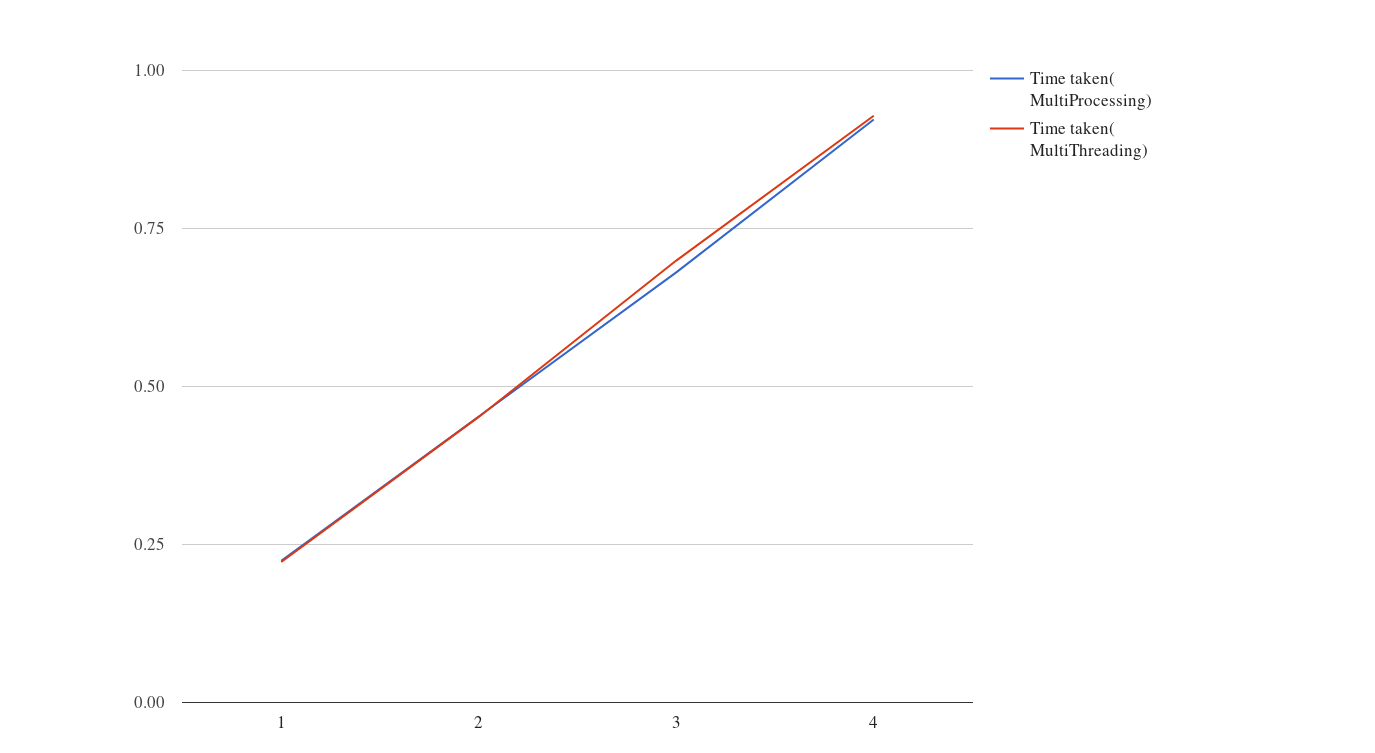
\includegraphics[width=200mm]{graph.png}
\caption{Comparision between time taken by MultiProcessing and Multithreading \label{overflow}}
\end{figure}
\end{document}